\documentclass[11pt]{article}
\usepackage[margin=0.83in]{geometry}
\usepackage[T1]{fontenc}
\usepackage{lmodern}
\usepackage{amsmath,amssymb,bm,booktabs,graphicx,microtype}
\usepackage[dvipsnames]{xcolor}
\usepackage[colorlinks=true,linkcolor=MidnightBlue,citecolor=MidnightBlue,urlcolor=MidnightBlue]{hyperref}
\usepackage{caption}
\usepackage{placeins}
\usepackage{enumitem}
\setlist{nosep}
\graphicspath{{../figures/}}
\setlength{\parskip}{0.35em}
\setlength{\parindent}{0pt}
\title{Stochastic diffraction in strongly lensed black-hole mergers\\[0.4em]
\large A reproducible perturbative calculation and a stellar-foreground check}
\author{Research calculation note}
\date{21 November 2026}

\begin{document}
\maketitle
\begin{abstract}
Strong lensing offers a physically motivated way to combine a high-redshift
gravitational-wave source with a high observed signal-to-noise ratio. It also
changes the response to small density fluctuations near a macroimage. We
implement the single-plane Born response of Oguri and Takahashi (2022), project
out ordinary magnification, phase, and arrival time, and calculate the full real
covariance of the differential waveform of a minimum/saddle image pair. The
calculation separates the known-realization residual SNR from the information
in an unknown stochastic covariance. Analytic power-law checks show that the
fractional signal can grow approximately linearly with magnification, in
addition to the usual square-root strain enhancement. An explicitly specified
NFW population illustrates this effect, but its predicted ground-band signal
remains smaller than the stellar foreground in the same benchmark. This is a
conditional calculation, not a calibrated CDM, detector, or merger-rate forecast.
\end{abstract}

\section{Results and interpretation}

\textbf{The idea is physically well motivated, and has direct prior art.}
Oguri and Takahashi~\cite{oguri2022} already derived the macroimage response
and proposed comparing repeated waveforms. Our contribution here is a
reproducible implementation with a bandwise nuisance projection, real joint
covariance, unequal-image noise accounting, and an explicit stellar-foreground
comparison. The recent stochastic-halo study~\cite{choi2026} and the strongly
lensed LISA calculations~\cite{ando2026a,ando2026b} motivate the application;
their LISA signal normalizations are not imported into a ground-based forecast.

The main results are:
\begin{enumerate}
\item At a fixed lens-plane convergence spectrum, a near-critical macroimage
enhances the \emph{fractional frequency-dependent} residual as well as the GW
strain. For $P_\kappa\propto k^{-2}$, a local fold-like image with eigenvalues
$(\pm1/|\mu|,1)$ has fractional RMS gain
$G\simeq\sqrt{3/8}|\mu|$ at large magnification. The known-residual SNR
therefore grows approximately as $|\mu|^{3/2}$ in this special model.
\item The differential measurement pays the noise of both images:
$\rho_\Delta=\rho_1\rho_2/(\rho_1^2+\rho_2^2)^{1/2}$ when the normalized
spectral weights agree. Repeating the waveform helps with intrinsic source
uncertainty; it does not eliminate the noise of the fainter image.
\item In our explicitly parameterized NFW benchmark over $10$--$100$ Hz,
the differential subhalo RMS is approximately $0.20\%$ at $|\mu|=30$ and
$0.81\%$ at $|\mu|=100$. These values depend on the local surface population,
concentrations, and frequency weighting.
\item The benchmark stellar differential RMS is approximately $3.3\%$ and
$5.9\%$ at the same magnifications. Marginalizing its random realization
reduces information about the weaker subhalo component. A detected modulation
cannot automatically be attributed to dark matter.
\item The earlier informal estimate of equal CDM diffraction in LISA and
ground-based bands is not supported by the actual plotted slope of
Ref.~\cite{choi2026}. A digitized slope implies a conditional RMS ratio nearer
$0.2$ for a four-decade frequency increase; see Section~\ref{sec:figure-audit}.
\end{enumerate}

These results favor studying high-magnification pairs with small stellar surface
density and useful low-frequency sensitivity. They do not establish how often
such pairs occur, whether their subhalos survive the lens environment, or whether
the Born approximation is accurate for the stellar field close to a caustic.

\begin{figure}[htbp]
\centering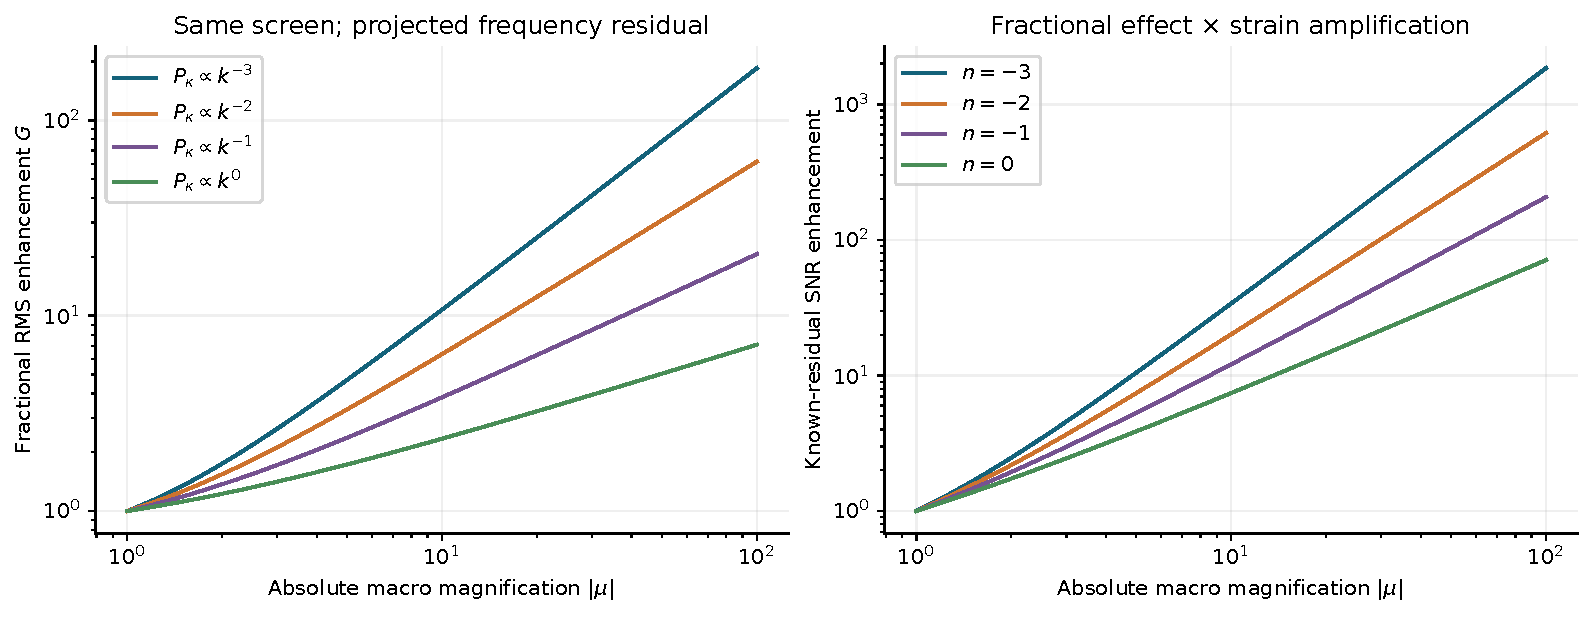
\includegraphics[width=\linewidth]{scale_free_enhancement.pdf}
\caption{Analytic conditional enhancement for isotropic power-law convergence
spectra. The left panel shows the fractional residual gain, after projection;
the right also includes the $\sqrt{|\mu|}$ strain gain. Here $n$ is the slope
of $P_\kappa$, not of power per logarithmic interval. These curves hold the
screen spectrum fixed and do not specify its astrophysical normalization.}
\end{figure}
\FloatBarrier

\section{Diffraction about a smooth macroimage}

We use the single-plane perturbative framework of
Oguri and Takahashi~\cite{oguri2022}.  The stochastic halo signal studied
by Choi et al.~\cite{choi2026} motivates the application, but none of the
normalizations below is calibrated to their line-of-sight CDM calculation.
All coordinates in this section are physical lens-plane coordinates.
For angular-diameter distances $D_l,D_s,D_{ls}$ and observed frequency $f$,
define
\begin{equation}
 r_F^2(f)=\frac{cD_lD_{ls}}{2\pi f(1+z_l)D_s},\qquad
 A=\begin{pmatrix}\lambda_1&0\\0&\lambda_2\end{pmatrix},\qquad
 |\mu|=\frac{1}{|\lambda_1\lambda_2|}.
\end{equation}
The eigenvalues may have either sign but must be nonzero.  Locally, the
smooth Fermat potential is quadratic.  Dividing its perturbed Fresnel
integral by the unperturbed one gives
\begin{equation}
 \frac{F}{F_0}=
 \frac{\displaystyle\int d^2x\,
  \exp\left[\frac{i\boldsymbol{x}^{T}A\boldsymbol{x}}{2r_F^2}
                -\frac{i\delta\psi(\boldsymbol{x})}{r_F^2}\right]}
 {\displaystyle\int d^2x\,
  \exp\left[\frac{i\boldsymbol{x}^{T}A\boldsymbol{x}}{2r_F^2}\right]}.
 \label{eq:macro-fresnel}
\end{equation}
The smooth factor has modulus $|F_0|=\sqrt{|\mu|}$ and the appropriate
Morse phase.  The perturbing potential obeys
$\nabla^2\delta\psi=2\delta\kappa$.
We remove the arrival-time shift $-\delta\psi(0)/r_F^2$ from the phase
and retain first order in $\delta\psi$.  With Fourier convention
$\delta\kappa(\boldsymbol{x})=
\int d^2k\,\widetilde\kappa(\boldsymbol{k})
e^{i\boldsymbol{k}\cdot\boldsymbol{x}}/(2\pi)^2$,
the Gaussian integral yields
\begin{align}
 \eta(f)&\equiv e^{i\delta\psi(0)/r_F^2}\frac{F(f)}{F_0(f)}-1
 =\int\frac{d^2k}{(2\pi)^2}\,
 \widetilde\kappa(\boldsymbol{k}) H_A(f,\boldsymbol{k}),\\
 H_A(f,\boldsymbol{k})&=
 \frac{2i}{r_F^2 k^2}
 \left\{\exp\left[-\frac{i r_F^2}{2}
 \boldsymbol{k}^{T}A^{-1}\boldsymbol{k}\right]-1\right\}.
 \label{eq:macro-kernel}
\end{align}
Equation~\eqref{eq:macro-kernel} is Eq.~(21) of
Ref.~\cite{oguri2022}, with their directional magnifications equal to
$\lambda_1^{-1},\lambda_2^{-1}$.  It applies to saddles as well as minima.
For $A=I$, $H=(1-e^{-is})/(is)$, where $s=r_F^2 k^2/2$.

The numerical implementation uses
$q=k r_F(f_{\rm ref})$, $f_{\rm ref}=100\,\mathrm{Hz}$, and
\begin{equation}
 b(\theta)=\frac{\cos^2\theta}{\lambda_1}
           +\frac{\sin^2\theta}{\lambda_2},\qquad
 s=\frac{q^2b(\theta)f_{\rm ref}}{2f},\qquad
 H_A=b(\theta)\,\frac{\sin(s/2)}{s/2}e^{-is/2}.
\end{equation}
This form is continuous at $q=0$ and $b=0$.  At fixed $\boldsymbol{k}$,
$H_A\to b(\theta)$ as $f\to\infty$: a real, frequency-independent
geometric magnification, not a measurable diffraction residual by itself.

\subsection{Projection and real covariance}

For normalized positive frequency weights $w_a$, the relevant inner
product is $\operatorname{Re}\sum_a w_a u_a^*v_a$.
The nuisance directions for an image or an aligned image ratio are
$1,i,if$, corresponding to amplitude, phase, and arrival time.  We project
the real part of $H$ off a constant and its imaginary part off a constant
plus a linear function of $f$:
\begin{align}
 \operatorname{Re}(QH)&=\operatorname{Re}H-
                  \langle\operatorname{Re}H\rangle_w,\\
 \operatorname{Im}(QH)&=\operatorname{Im}H-
                  \langle\operatorname{Im}H\rangle_w
 -(f-\langle f\rangle_w)
  \frac{\langle(f-\langle f\rangle_w)\operatorname{Im}H\rangle_w}
       {\langle(f-\langle f\rangle_w)^2\rangle_w}.
 \label{eq:real-projection}
\end{align}
Complex regression on $\{1,f\}$ would also discard a real amplitude
slope and would therefore remove a physical mode unnecessarily.

Define the homogeneous convergence spectrum by
$\langle\widetilde\kappa(\boldsymbol{k})
\widetilde\kappa^*(\boldsymbol{k}')\rangle
=(2\pi)^2\delta^{(2)}(\boldsymbol{k}-\boldsymbol{k}')P_\kappa(k)$
and $\Delta_\kappa^2(k)=k^2P_\kappa(k)/(2\pi)$.
Writing
$\boldsymbol{v}(k,\theta)=[\operatorname{Re}(QH),
\operatorname{Im}(QH)]^T$, the unweighted joint covariance is
\begin{equation}
 C=\int d\ln k\,\Delta_\kappa^2(k)
       \left\langle\boldsymbol{v}\boldsymbol{v}^{T}\right\rangle_\theta.
 \label{eq:real-covariance}
\end{equation}
The mean-square projected fractional residual is
$\sigma_\perp^2=\operatorname{tr}(WC)$ with
$W=\operatorname{diag}(w_1,\ldots,w_N,w_1,\ldots,w_N)$.
The real field makes the complex fluctuations noncircular; the joint
real covariance retains information lost by keeping only
$\langle\eta\eta^*\rangle$.

For two images, the cross-covariance before projection includes
$H_{A_1}(f,\boldsymbol{k})H_{A_2}^*(g,\boldsymbol{k})
e^{i\boldsymbol{k}\cdot(\boldsymbol{x}_1-\boldsymbol{x}_2)}$.
Their differential covariance is $C_1+C_2-C_{12}-C_{21}$.
Using $C_1+C_2$ therefore requires independent image perturbations;
it is not automatic for all line-of-sight structures.

\subsection{An analytic power-law check}

Suppose $P_\kappa(k)=C_0 k^n$ on all relevant scales.  Consider a fixed
fractional frequency band $f=f_0 u$ with identical weights as a function
of $u$.  Changing radial variable to
$p=k r_F(f_0)\sqrt{|b(\theta)|}$ in
Eq.~\eqref{eq:real-covariance} gives
\begin{equation}
 \sigma_\perp^2(f_0,A)\ \propto\
 f_0^{(n+2)/2}
 \left\langle |b(\theta)|^{(2-n)/2}\right\rangle_\theta,
 \qquad -6<n<2.
 \label{eq:powerlaw-scaling}
\end{equation}
The convergence range follows from $QH=O(k^2)$ at small $k$ and
$QH=O(k^{-2})$ at large $k$.  Thus the RMS scales as
$f_0^{(n+2)/4}$.  Frequency independence occurs only for $n=-2$;
it is not a general prediction for CDM or for two detectors with
different waveform and noise weights.

For $n=-2$, the RMS gain relative to $A=I$ has the closed form
\begin{equation}
 G^2\equiv\frac{\sigma_\perp^2(A)}{\sigma_\perp^2(I)}
 =\left\langle b^2\right\rangle_\theta
 =\frac{3}{8}\left(\lambda_1^{-2}+\lambda_2^{-2}\right)
   +\frac{1}{4\lambda_1\lambda_2}.
 \label{eq:flat-spectrum-gain}
\end{equation}
For $\lambda_2=1$ and $\lambda_1=\pm1/|\mu|$,
$G\simeq\sqrt{3/8}\,|\mu|$ at large $|\mu|$.
This fractional enhancement is separate from the smooth-waveform SNR
gain $\sqrt{|\mu|}$.  The radial and angular numerical integrals are
tested against Eq.~\eqref{eq:flat-spectrum-gain}; finite spectral cutoffs
and changes of slope require the full integral.

\paragraph{Scope and validity.}
These results describe a weak screen at the main lens plane and a
locally quadratic, nonsingular macroimage.  The elliptical Fresnel
widths $r_F/\sqrt{|\lambda_i|}$ must remain within that local region,
and perturbations must remain small enough for the Born expansion.
One cannot apply the same $A^{-1}$ to every foreground and background
screen: their coupling to the macro lens needs a multiplane propagation
calculation.  The calculation also does not follow newly created
microimages or nonlinear caustics.  Stellar fluctuations can dominate
CDM fluctuations in the ground-based band even when both are enhanced
by strong lensing~\cite{oguri2022}.

\section{What two lensed images actually measure}
\label{sec:inference}

This section derives the idealized two-image likelihood used in our sensitivity
calculations. The weak-diffraction signal is a random frequency-dependent
perturbation, as in the framework of \cite{oguri2022,choi2026}; the differential
weights, nuisance projection, and statistical information accounting below are
derived here. The results are sensitivity requirements, not population forecasts.

\subsection{Eliminating a shared waveform and paying its noise cost}

For positive Fourier frequencies, write the two scalar observations as
\begin{equation}
 d_i(f)=\sqrt{|\mu_i|}\,e^{i(2\pi f t_i+\phi_i)}
 h(f)[1+\delta_i(f)]+n_i(f),\qquad i=1,2.
\end{equation}
Here \(h\) is the common unlensed waveform, \(\delta_i\) is a fractional
perturbation, and the independent noises have one-sided power spectral densities
\(S_i(f)\). Dividing out the macro amplitude and phase and differencing removes
the common waveform at zeroth order:
\begin{equation}
 r(f)=h(f)[\delta_1(f)-\delta_2(f)]+n_\Delta(f),\qquad
 S_\Delta(f)=\frac{S_1(f)}{|\mu_1|}+\frac{S_2(f)}{|\mu_2|}.
\end{equation}
Define image SNR densities \(w_i(f)=4|\mu_i||h(f)|^2/S_i(f)\), with
\(\rho_i^2=\int w_i(f)\,df\). The exact differential weight is
\begin{equation}
 \boxed{w_\Delta(f)=\frac{4|h(f)|^2}{S_\Delta(f)}
 =\frac{w_1(f)w_2(f)}{w_1(f)+w_2(f)}.}
 \label{eq:infer_harmonic}
\end{equation}
This also follows by minimizing a two-image Gaussian likelihood over an
arbitrary common complex source amplitude independently in each frequency bin.
Thus source-waveform cancellation has a definite noise cost.

If the two SNR densities have identical normalized frequency dependence,
\(w_i(f)=\rho_i^2p(f)\), where \(\int p(f)\,df=1\), then
\begin{equation}
 \rho_\Delta\equiv\left[\int w_\Delta(f)\,df\right]^{1/2}
 =\frac{\rho_1\rho_2}{\sqrt{\rho_1^2+\rho_2^2}}.
 \label{eq:infer_rhodelta}
\end{equation}
Two equally loud images give \(\rho_\Delta=\rho_i/\sqrt{2}\); for unequal
images the quieter image limits the comparison. Equation~\eqref{eq:infer_rhodelta}
is an upper bound at fixed integrated image SNRs if their spectral shapes differ;
in that case one must first integrate Eq.~\eqref{eq:infer_harmonic}.

This scalar cancellation presumes that detector responses have been accounted
for. At different arrival times a real network measures different mixtures
\(F^+_I(t_i)h_++F^\times_I(t_i)h_\times\). Precession or higher harmonics can
make the polarization ratio frequency dependent. A realistic analysis should
therefore use a joint network likelihood sharing both source polarizations, or
propagate the uncertainty of a polarization reconstruction. A saddle image also
requires the actual Morse/Hilbert-transform operator: its phase is \(-i\) at
positive frequency and \(+i\) at negative frequency, up to Fourier convention.
For general waveforms this is not equivalent to shifting the binary's orbital
coalescence phase. Intrinsic waveform errors can cancel in a consistent joint
comparison; calibration and response errors need their own nuisance model.

\subsection{Projecting out ordinary magnification, phase, and delay}

Macro amplitudes and arrival times are fitted from the same data. Introduce the
real inner product
\begin{equation}
 (u,v)_\Delta=\operatorname{Re}\int df\,w_\Delta(f)u^*(f)v(f)
\end{equation}
and the three nuisance functions \(b_a(f)=\{1,i,2\pi if\}\), with real
coefficients. With \(\Gamma_{ab}=(b_a,b_b)_\Delta\), the retained perturbation is
\begin{equation}
 P_\perp u=u-\sum_{ab}b_a(\Gamma^{-1})_{ab}(b_b,u)_\Delta.
 \label{eq:infer_projection}
\end{equation}
A real rather than complex projection matters: a time shift removes an imaginary
linear slope, not a real amplitude slope. Fitting an arbitrary constant phase is
a conservative choice even if a Morse phase is theoretically discrete.

For \(\Delta\delta=\delta_1-\delta_2\), define the detector-weighted,
projected \emph{differential} fractional RMS by
\begin{equation}
 \epsilon_\Delta^2=\rho_\Delta^{-2}
 \int df\,w_\Delta(f)|P_\perp\Delta\delta(f)|^2.
\end{equation}
For a specified residual realization, its matched-filter SNR is
\begin{equation}
 \boxed{\rho_{\rm res}=\rho_\Delta\epsilon_\Delta.}
 \label{eq:infer_known}
\end{equation}
This is a useful sensitivity ceiling when the realization is not known; it is
not automatically the significance for discovering a stochastic covariance.
For example, two images each with \(\rho_i=500\) give
\(\rho_{\rm res}=3.54\) for \(\epsilon_\Delta=10^{-2}\), or \(0.354\) for
\(10^{-3}\). These are illustrative sensitivity inputs, not predicted CDM
residual amplitudes or event rates.

If each image instead has projected RMS \(\epsilon\), and their weighted real
correlation is \(c\), then
\begin{equation}
 \epsilon_\Delta^2=2\epsilon^2(1-c).
\end{equation}
For equally loud independent images, the extra \(\sqrt{2}\) differential signal
compensates the extra \(\sqrt{2}\) noise, yielding
\(\rho_{\rm res,rms}=\rho_i\epsilon\). A perfectly common perturbation cancels.
The experiment measures differential small-scale structure, and cannot retain
every mode of the total line-of-sight variance.

\subsection{Stochastic detection is a covariance problem}

The complex covariance of the difference is
\begin{equation}
 C_\Delta=C_{11}+C_{22}-C_{12}-C_{21},\qquad
 C_{ij}(f,f')=\langle\delta_i(f)\delta_j^*(f')\rangle.
\end{equation}
One must also retain the nonconjugated covariance
\(J_{ij}(f,f')=\langle\delta_i(f)\delta_j(f')\rangle\), or directly construct
the covariance of the stacked real and imaginary components. A real convergence
field with a complex diffraction kernel does not generally produce a proper,
circular complex process. Our implementation constructs the real covariance,
projects it with Eq.~\eqref{eq:infer_projection}, and whitens it using the
frequency weights. The resulting eigenvalues \(\eta_a\geq0\) are signal-variance
to noise-variance ratios in independent real modes.

On the retained whitened subspace, take \(x\sim N(0,I+\Lambda)\), where
\(\Lambda\) is the lens covariance and \(\eta_a\) are its eigenvalues. Integrating
over a Gaussian random lens realization gives
\begin{equation}
 \ln\frac{p(x|\Lambda)}{p(x|0)}=
 -\frac12\ln\det(I+\Lambda)
 +\frac12x^T[I-(I+\Lambda)^{-1}]x.
\end{equation}
Our covariance-information measure is
\begin{equation}
 \boxed{d\equiv\sqrt{2D_{\rm KL}(p_\Lambda\Vert p_0)}
 =\left\{\sum_a[\eta_a-\ln(1+\eta_a)]\right\}^{1/2}.}
 \label{eq:infer_KL}
\end{equation}
This is \emph{not a calibrated Gaussian discovery significance}. The expected
squared matched-filter SNR if the realization were known is instead
\(\langle\rho_{\rm res}^2\rangle=\sum_a\eta_a\).
For weak covariance, \(\eta_a\ll1\) for all modes,
\begin{equation}
 d^2\simeq \frac12\sum_a\eta_a^2,
\end{equation}
which is also the squared mean shift of the optimal quadratic score in units of
its null standard deviation. At fixed total residual power, spreading that
power over more independent weak modes reduces this covariance discrimination.

Kullback--Leibler divergences add for independent events. Thus \(N\) identical
events have \(d_N=\sqrt{N}\,d_1\). Because weak-signal covariance is proportional
to fractional amplitude squared, \(d\propto\epsilon^2\), the detectable
stochastic RMS amplitude improves only as \(N^{-1/4}\) in this regime. The
\(N^{-1/2}\) amplitude scaling of a known deterministic waveform does not apply
to independent unknown lens realizations. This Gaussian treatment is an
explicit approximation; a sparse, non-Gaussian halo population would require
an appropriate hierarchical likelihood.

\section{Detector-systematics checks and image-dependent waveform phases}
\label{sec:systematics}

Repeated images provide useful consistency tests, but not a universal proof
that a frequency-dependent residual is astrophysical. The distinction is between
calibration that is stable between images, calibration that changes differently
in different instruments, and an epoch-dependent error common to the network.

\subsection{Apply the Morse operator before differencing}

In geometric optics, a macroimage contributes
\begin{equation}
 \widetilde h_i(f)=\sqrt{|\mu_i|}\,e^{2\pi ift_i}
 M_{n_i}(f)[1+\delta_i(f)]\widetilde h(f),\qquad
 M_n(f)=e^{-i\pi n\,\operatorname{sgn}f},
 \label{eq:sys_morse}
\end{equation}
using a convention in which a delay gives \(e^{2\pi ift_i}\).
The Morse index is \(n=0,1/2,1\) for a minimum, saddle, and maximum of
the arrival-time surface, respectively \cite{dai2017}. At nonzero frequencies,
\begin{center}
\begin{tabular}{lll}
Image type & Fourier operator & Effect on real strain \\
\hline
Minimum & \(1\) & unchanged \\
Saddle & \(-i\operatorname{sgn}f\) & Hilbert transform \\
Maximum & \(-1\) & overall sign reversal
\end{tabular}
\end{center}
Thus a saddle is not simply a sign-reversed waveform. Negative signed
magnification denotes image parity; the strain amplitude is
\(\sqrt{|\mu|}\), while its Morse phase is supplied separately. A maximum
has positive parity and nevertheless reverses the strain sign.
The relation \(M_n(-f)=M_n(f)^*\) preserves a real time-domain signal.
The zero-frequency geometric-optics limit is outside this calculation.

Before comparison, divide each image by its magnification and delay and apply
\(M_{n_i}^*(f)\). This removes the entire image operator, including for signals
with higher harmonics. Treating a saddle as a binary coalescence-phase shift is
not generally valid. An uncorrected Morse phase can otherwise produce a large
spurious residual. The fractional perturbation \(\delta_i\) remaining after
this correction has no universal sign; its amplitude and phase depend on the
perturbing structure and macroimage response \cite{oguri2022}.

The parity correction is not a free systematic-error reversal. A multiplicative
calibration error acts on the phase-shifted GW itself, so applying the inverse
Morse operator also rotates that error with the signal. After alignment, the
residual still contains $h[(\delta_i-\delta_j)+(c_{Ii}-c_{Ij})]$.
Image parity therefore helps identify and align lensed images; it does not
by itself distinguish diffraction from multiplicative calibration drift.

\subsection{Use independent detector observations of the same residual}

For a known sky direction, the network signal at each epoch can be written
\(\boldsymbol d_i=R_i[F_i\boldsymbol h]+\boldsymbol n_i\), where \(R_i\)
maps the two source polarizations into detector strains. At the scalar-lensing
order used here, \(F_i(f)\) multiplies both polarizations and is common to all
detectors observing that image. It therefore remains in the same two-polarization
signal subspace even if its frequency dependence is complicated. A noise-weighted
null projector satisfies
\begin{equation}
 Q_iR_i=0,\qquad Q_iR_i[F_i\boldsymbol h]=0.
\end{equation}
The null stream contains detector noise rather than the lensed GW. An
instrument-specific calibration error or glitch will generally leak into it.
This is the standard redundant-network consistency test
\cite{wenschutz2005,schutz2020}; it requires sufficient independent detector
responses and correct timing, sky location, and response modeling.

Image-to-image differencing supplies an additional check. For illustration,
suppose detector/polarization responses and the macro operators have been
corrected so that each scalar channel obeys
\begin{equation}
 x_{Ii}(f)=g_{Ii}(f)F_i(f)h(f),\qquad g_{Ii}=1+c_{Ii},
 \label{eq:sys_scalar}
\end{equation}
temporarily omitting additive noise. This is a model for response-corrected
channels, not a prescription for dividing raw strains whose antenna mixtures
change as Earth rotates. The image ratio in detector \(I\) is
\begin{equation}
 R_I^{ij}=\frac{x_{Ii}}{x_{Ij}}
 =\frac{F_i}{F_j}\frac{g_{Ii}}{g_{Ij}}.
\end{equation}
An arbitrary frequency-dependent calibration \emph{stable between epochs},
\(g_{Ii}=g_{Ij}\), cancels exactly. To first order,
\(R_I^{ij}-1=\delta_i-\delta_j+c_{Ii}-c_{Ij}\).
Taking the difference of this quantity between instruments cancels the lensing
signal and tests detector-dependent calibration evolution.

A division-free exact version for instruments \(I,J\) is the determinant
\begin{equation}
 \mathcal N_{IJ}^{ij}=x_{Ii}x_{Jj}-x_{Ij}x_{Ji}
 =F_iF_jh^2(g_{Ii}g_{Jj}-g_{Ij}g_{Ji}).
 \label{eq:sys_crossdifference}
\end{equation}
It vanishes for stable detector calibration even when the two images have
different diffraction. Its noise covariance must be propagated; in actual
analysis, fit the equivalent joint likelihood rather than divide noisy Fourier
bins. Agreement between detector-specific differential residuals, together with
a noise-consistent null stream, is strong evidence against an error confined to
one instrument.

\subsection{The remaining degeneracy is exact}

An epoch-dependent transfer \(a_i(f)\) common to every detector cannot be
separated from lensing by these tests. The transformation
\begin{equation}
 F_i(f)\longrightarrow a_i(f)F_i(f),\qquad
 g_{Ii}(f)\longrightarrow g_{Ii}(f)/a_i(f)
\end{equation}
leaves every measured strain unchanged. Such a common multiplicative error
passes the null stream and Eq.~\eqref{eq:sys_crossdifference}. External calibration
information and calibration priors remain necessary; a static common error
does cancel between images, but one that changes between their arrivals does not.

Physical diffraction templates also predict correlated amplitude and phase
structure and frequency coherence \cite{oguri2022}. Testing those predictions,
and checking that the same transfer acts on both polarizations, adds evidence.
Neither a smooth residual nor Hermitian symmetry \(F(-f)=F(f)^*\) is unique to
lensing: a physical detector transfer can satisfy both. There is no universal
minimum-phase amplitude--phase test for a multipath lens. Likewise,
\(R^{12}R^{23}R^{31}=1\) for three ratios formed from the same data is an
algebraic identity, not an independent lensing or calibration test.

\subsection{A joint amplitude--phase consistency relation}
\label{sec:kernel-consistency}

The lensing response constrains amplitude and phase jointly.  In
particular, a power-spectrum-independent variance relation was established
for weak lensing by Inamori and Suyama~\cite{inamori2021} and extended to
weak perturbations of a fixed strong lens by Nakazono and
Suyama~\cite{nakazono2026}.  In the single-plane Born model used here,
the underlying identity follows directly from the kernel of
Oguri and Takahashi~\cite{oguri2022}:
\begin{equation}
 H_A(f,k,\theta)=b(\theta)
 \frac{\sin s+i(\cos s-1)}{s},\qquad
 s=\frac{r_F^2(f)k^2b(\theta)}{2}.
\end{equation}
Since $r_F^2(2f)=r_F^2(f)/2$, elementary trigonometry gives
\begin{equation}
 |H_A(f,k,\theta)|^2
 =\frac{4b(\theta)^2\sin^2(s/2)}{s^2}
 =\left[\operatorname{Re}H_A(2f,k,\theta)\right]^2.
 \label{eq:modewise-consistency}
\end{equation}
The result includes saddles; $b$ need not be positive.  Integrating
against any nonnegative homogeneous convergence power spectrum yields,
to leading nonzero order in the perturbation,
\begin{equation}
 \left\langle K(f)^2\right\rangle+
 \left\langle S(f)^2\right\rangle
 =\left\langle K(2f)^2\right\rangle,
 \label{eq:ensemble-consistency}
\end{equation}
where $K=\operatorname{Re}\eta$ and $S=\operatorname{Im}\eta$ at first
order, after removing the geometric arrival-time phase.  More generally,
the quantities in Ref.~\cite{nakazono2026} are defined through the
logarithm of the amplification factor; their leading variances agree
with those used here.  The brackets average over weak perturbations at
fixed macro lens.  The code tests Eq.~\eqref{eq:modewise-consistency}
directly, including negative-parity cases.

Nakazono and Suyama~\cite{nakazono2026} also obtain, through second
order in the weak potential and with the smooth macro lens held fixed,
\begin{equation}
 \langle S(f)\rangle-\tfrac12\langle S(2f)\rangle
   =-\langle K(f)S(f)\rangle,\qquad
 \langle K(f)\rangle=-\langle K(f)^2\rangle.
\end{equation}
Here $F_j/F_{j,0}=\exp[K_j+i(S_j+2\pi f\Delta t_j)]$ defines the
logarithmic amplitude and the delay-subtracted phase.  Within their
geometric macro-lens and Limber treatment, they additionally derive
$\langle e^{2K_j}\rangle=1$ beyond the perturbative expansion.
Our first-order covariance calculation does not predict the second-order
means; testing these identities requires a consistently extended
propagation calculation and the same ensemble definition.  They cannot
be applied unchanged to projected image differences.

Three limitations matter observationally.  First, the relation holds
for ensemble moments, not the squared residual of one realization:
cross terms between different Fourier modes cancel in the ensemble,
not in each event.  Second, our detector-weighted projection $Q$ removes
amplitude, phase, and delay using a finite frequency band.  It does not
preserve Eq.~\eqref{eq:ensemble-consistency}; a valid test must pass the
theoretical joint covariance through the same projection, frequency
window, and noise weighting as the data.  Third, independent image
residuals can have their variances added, but cross-correlated images
with different macro kernels introduce cross terms that need not obey
the simple relation.  It would therefore be incorrect to apply it
unchanged to a measured, projected image difference.

These relations restrict a lensing model, but do not identify lensing
uniquely.  A multiplicative detector response can also create correlated
amplitude and phase errors.  Stronger evidence requires a common
astrophysical transfer function across independent detectors, consistency
with lens geometry and image parity, and calibration information.

\paragraph{Causality and image ratios.}
Kramers--Kronig relations constrain the full physical lens transfer
function when its time origin is fixed at the earliest arrival.
They follow from causality~\cite{tanaka2023} but cannot automatically
be imposed on the normalized ratio $F_1/F_2$:
division introduces the zeros of $F_2$ as possible poles, and the inverse
response need not be causal.  An isolated, infinite quadratic saddle
model also has no lower bound on its local Fermat time, so it does not
by itself supply the global causal transfer function.  Finite-band
projection changes the relation further.  Finally, recovering phase
from magnitude requires any zero-dependent all-pass contributions
\cite{suyama2025}, and
causal instrumental filters can obey dispersion relations too.  Thus
causality is a physical consistency requirement, not a unique detector
systematics veto.

\begin{figure}[htbp]
\centering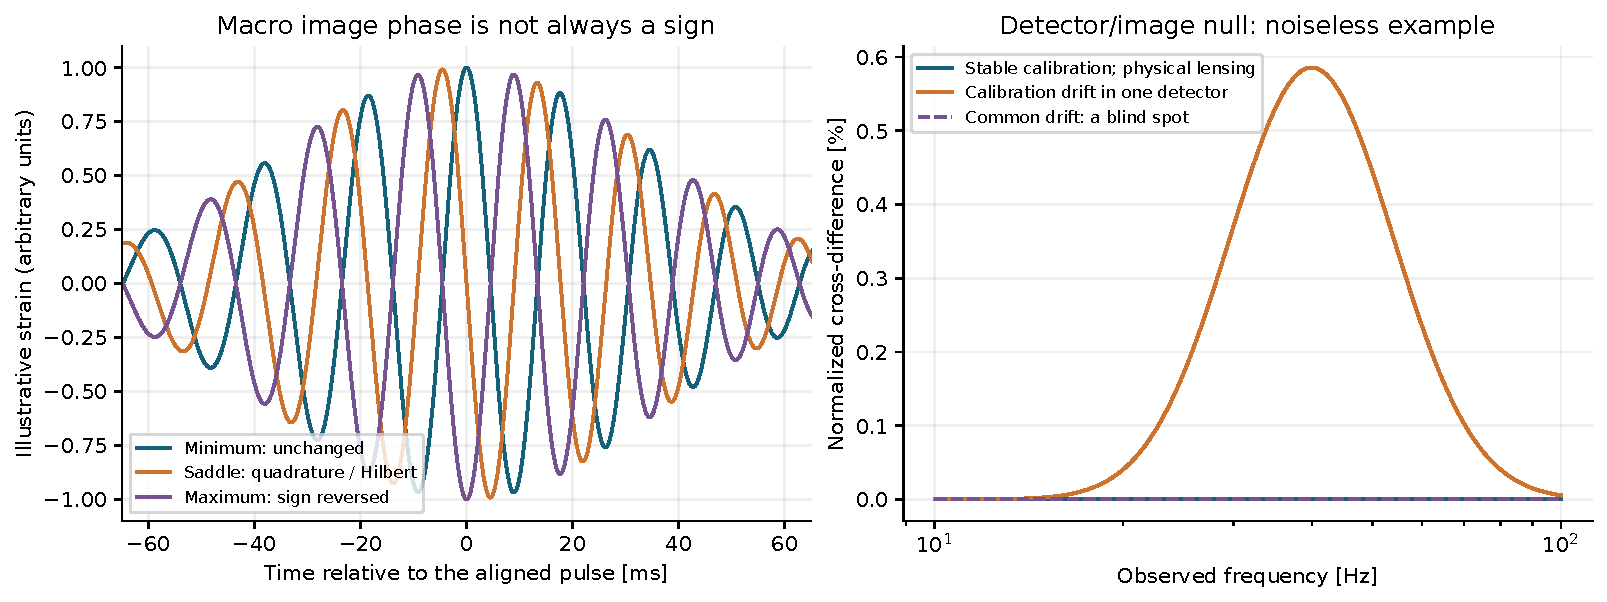
\includegraphics[width=\linewidth]{morse_and_systematics.pdf}
\caption{Left: the three geometric image operators applied to an illustrative
band-limited chirp, not a black-hole waveform model. Right: a noiseless
image/detector cross-difference rejects detector-specific drift while retaining
its exact blind spot to drift common to all detectors. Its normalization is
for visualization only; no noise or significance calculation is implied.}
\end{figure}
\FloatBarrier

\section{An explicit local subhalo and stellar benchmark}
\label{sec:model}

We choose a flat matter--Lambda geometry with $H_0=70\,\mathrm{km\,s^{-1}\,Mpc^{-1}}$,
$\Omega_m=0.3$, lens redshift $z_l=0.5$, and source redshift $z_s=2$.
All distances, projected surface densities, and wavenumbers in the implementation
are physical. The resulting critical surface density and Fresnel scale are
\begin{equation}
 \Sigma_{\rm cr}=\frac{c^2D_s}{4\pi G D_lD_{ls}}
 \simeq2079\,M_\odot\,\mathrm{pc^{-2}},\qquad
 r_F(100\,\mathrm{Hz})\simeq0.0908\,\mathrm{pc}.
\end{equation}
The elongated Fresnel width is $r_F\sqrt{|\mu|}$ for the chosen unit radial
eigenvalue. At $100$ Hz it is about $0.91$ pc for $|\mu|=100$.
This spatial scale does not imply a unique halo mass: an extended halo's
profile, abundance, and impact parameter all enter its diffraction signal.

\subsection{Finite NFW profiles and a surface population}

Take an unclustered local surface-number distribution
$d^2N/(dA\,dM)=B M^{-\alpha}$, with
\begin{equation}
 \alpha=1.9,\quad M_{\min}=10^{-6}M_\odot,\quad
 M_{\max}=10^8M_\odot,\quad
 \int dM\,M\frac{d^2N}{dA\,dM}=\kappa_{\rm sub}\Sigma_{\rm cr},
 \quad \kappa_{\rm sub}=0.005.
\end{equation}
Each halo is truncated at $r_{200}$, defined with respect to $200\rho_c(z_l)$,
and normalized to finite mass $M$. Its concentration is an explicit input:
\begin{equation}
 c_{200}(M)=\min\left[200,\ c_6\left(\frac{M}{10^6M_\odot}\right)^{-0.1}\right],
 \qquad c_6=15,30,60,
 \label{eq:concentration-model}
\end{equation}
with $c_6=30$ the benchmark. These are exploratory concentration choices,
not fitted relations. In particular, the model does not include stripping,
subhalo depletion, a radial distribution within a host, or a tidal history.

The normalized transform of the projected profile equals the three-dimensional
spherical transform evaluated at transverse wavenumber. With $x=kr_s$ and
$g(c)=\ln(1+c)-c/(1+c)$, it is
\begin{align}
 u(x,c)=\frac{1}{g(c)}\bigg\{&\sin x\,[\operatorname{Si}((1+c)x)-\operatorname{Si}(x)]
 +\cos x\,[\operatorname{Ci}((1+c)x)-\operatorname{Ci}(x)]\nonumber\\
 &-\frac{\sin(cx)}{(1+c)x}\bigg\},\qquad u(0,c)=1.
\end{align}
The Poisson convergence spectrum is
\begin{equation}
 P_{\kappa,\rm sub}(k)=\int dM\,\frac{d^2N}{dA\,dM}
 \left(\frac{M}{\Sigma_{\rm cr}}\right)^2 |u(kr_s,c)|^2.
 \label{eq:subhalo-power}
\end{equation}
This is the standard shot-spectrum construction used in
Ref.~\cite{oguri2022}; our population and truncation prescription are separately
specified, so this is not a reproduction of that paper's figures.

The $A=I$ comparison keeps this same nonzero fluctuation spectrum as a
mathematical reference filter. It is not a self-consistent zero-convergence
lens galaxy. Similarly, the magnification sweep varies the Jacobian while
holding local stellar and subhalo populations fixed; it is a response study,
not a family of fully solved galaxy lenses.

\subsection{Stellar shot noise and its limits}

The point-mass benchmark uses
\begin{equation}
 P_{\kappa,\star}=\frac{\kappa_\star M_{\rm eff}}{\Sigma_{\rm cr}},\qquad
 M_{\rm eff}=\frac{\langle M^2\rangle}{\langle M\rangle}=0.5M_\odot,
 \qquad\kappa_\star=0.025.
 \label{eq:stellar-power}
\end{equation}
For a near-critical region with total convergence near $0.5$, this corresponds
to an illustrative stellar fraction of $5\%$ and subhalo fraction of $1\%$.
We also rescale the stellar covariance to $\kappa_\star=0$, $0.00025$, and
$0.0025$ to show environmental sensitivity. A real stellar mass function,
remnants, and nonlinear microlensing are not implemented. The importance of
such fields for strongly lensed GWs has also been studied explicitly in
Ref.~\cite{zumalacarregui2026}.

For a point mass, $w_M=8\pi GM(1+z_l)f/c^3$. At $100$ Hz and
$M=0.5M_\odot$, $w_M=0.00928$ in this geometry, but
$|\mu|w_M\simeq0.93$ for $|\mu|=100$.
This is a warning that proximity to the macrocritical curve can defeat a
naive weak-stellar-screen approximation; it is not a complete validity test.
The largest-magnification stellar numbers are therefore diagnostic benchmarks,
not validated nonlinear microlensing predictions.

\begin{figure}[htbp]
\centering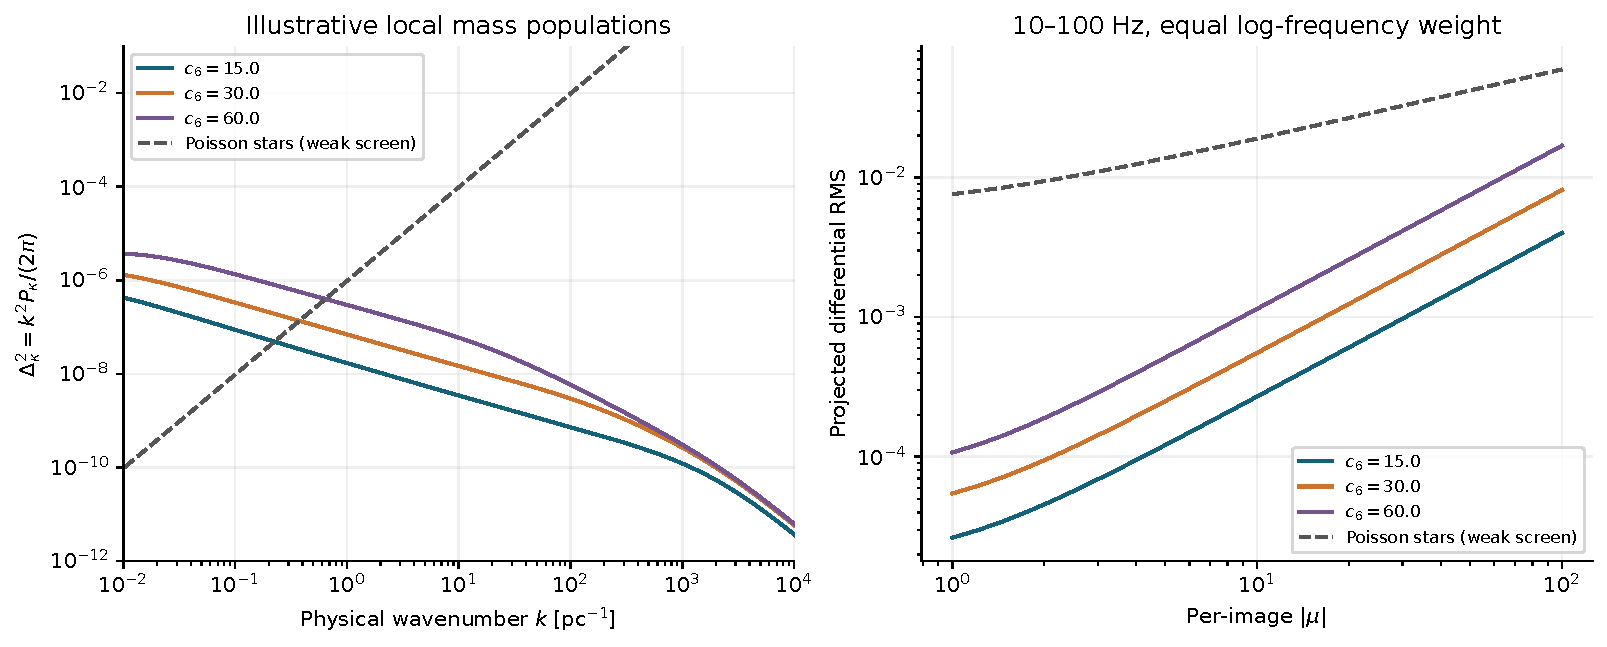
\includegraphics[width=\linewidth]{local_population_comparison.pdf}
\caption{An explicitly specified, local, physical population. The left panel
shows the convergence power; the right shows the projected RMS of independent
minimum and saddle image perturbations. Concentration choices bracket one
important uncertainty. Dashed stellar curves use the weak-screen shot spectrum;
they are not microlensing-map simulations.}
\end{figure}

\subsection{Band weights and high-redshift binaries}

The default calculation uses 64 logarithmically spaced observed frequencies
from $10$ to $100$ Hz and equal weight per $d\ln f$, with trapezoidal endpoint
weights. The input $\rho_0$ is the unlensed SNR of \emph{one source in that
specified band and detector/network convention}. It is not a total SNR from
a different band. We do not assume a particular Einstein Telescope, Cosmic
Explorer, or unspecified fourth-generation sensitivity curve.

For comparison, we implement $3$--$30$ Hz and $30$--$300$ Hz bands and a second
weight proportional to $f^{-7/3}df$, corresponding to Newtonian inspiral in
white strain noise. At $|\mu|=30$, the benchmark differential subhalo RMS is
approximately $2.44$, $1.99$, and $1.66$ times $10^{-3}$ in the three log-weighted
bands. The $10$--$100$ Hz white-noise inspiral weight gives $1.79\times10^{-3}$.
These are sensitivity checks, not detector response models.

Redshift changes which band contains the waveform. For example, the test-particle
ISCO reference is $f_{\rm ISCO}=c^3/[6^{3/2}\pi G(1+z_s)M]$;
a source-frame $30+30M_\odot$ binary at $z_s=2$ gives about $24$ Hz.
Merger and ringdown extend above that reference. Thus a physical detector
forecast must use a redshifted inspiral--merger--ringdown waveform, rather than
assigning a universal $30$--$300$ Hz weight to all high-redshift binaries.

\begin{figure}[htbp]
\centering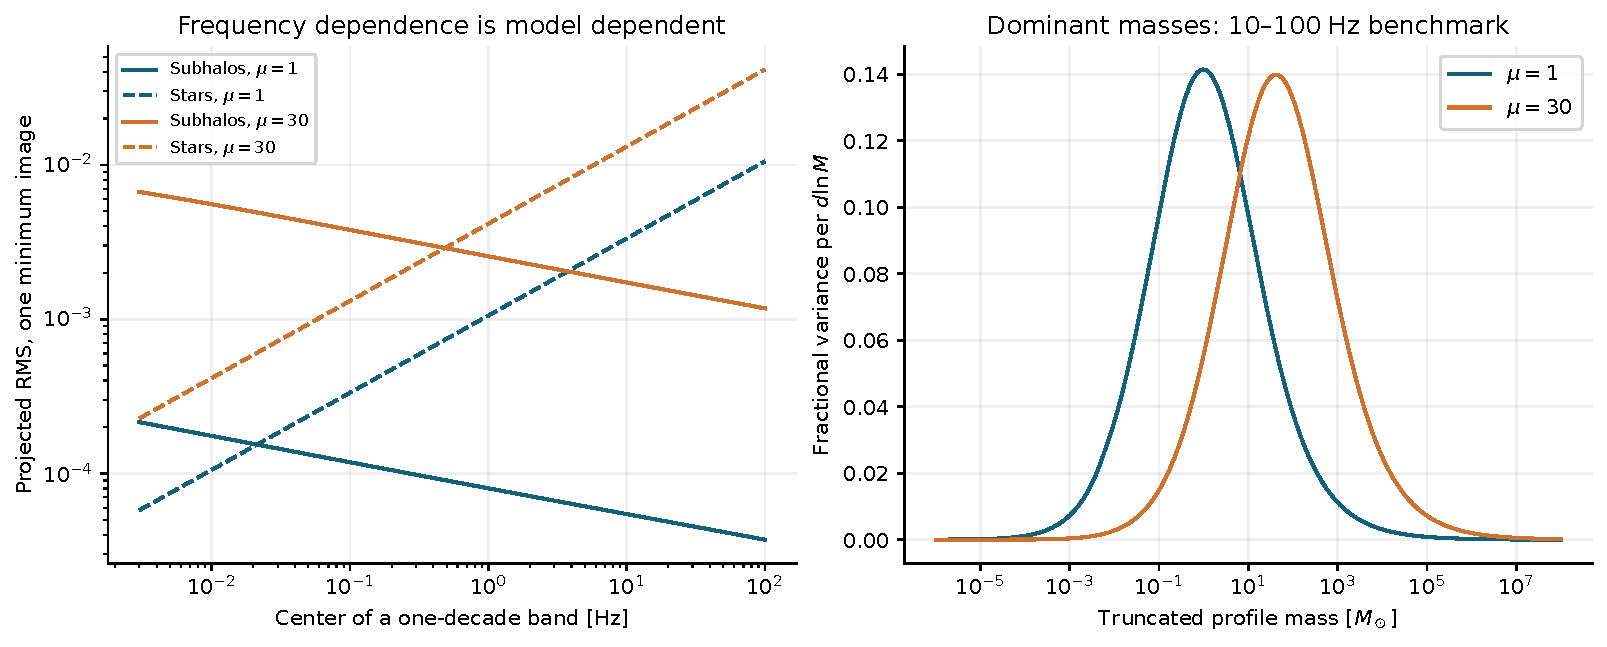
\includegraphics[width=\linewidth]{frequency_and_mass_dependence.pdf}
\caption{Left: moving a one-decade band changes both the halo and stellar
residuals in the explicit benchmark. Right: the contribution to variance per
logarithmic halo mass in the $10$--$100$ Hz minimum-image calculation, normalized
to unit area. The halo mass at which a low-mass cut saturates is not necessarily
the mass that dominates the signal.}
\end{figure}
\FloatBarrier

\section{Numerical differential sensitivity}

Consider independent minimum and saddle fluctuations with equal absolute
magnification and eigenvalues $(1/|\mu|,1)$ and $(-1/|\mu|,1)$.
The observed SNR of each image is $\rho_i=\sqrt{|\mu|}\rho_0$.
For the finite local population above, Table~\ref{tab:bench} gives the result
for $\rho_0=50$. Only the environment and frequency-band assumptions turn the
dimensionless sensitivity requirements into these illustrative numbers.

\begin{table}[htbp]
\centering\small
% Generated by scripts/run_calculations.py; do not edit.
\begin{tabular}{rrrrrr}
\toprule
$|\mu|$ & $\rho_0$ & $\rho_{\rm image}$ & $\epsilon_{\Delta,{\rm DM}}$ & $\rho_{\rm res,rms}$ & $d_{\rm DM|stars}$ \\
\midrule
1 & 50 & 50 & 5.46e-05 & 0.002 & 0.000 \\
10 & 50 & 158 & 5.55e-04 & 0.062 & 0.001 \\
30 & 50 & 274 & 1.99e-03 & 0.386 & 0.007 \\
100 & 50 & 500 & 8.14e-03 & 2.876 & 0.054 \\
\bottomrule
\end{tabular}

\caption{Default $10$--$100$ Hz local benchmark. The residual SNR is an
RMS \emph{known-realization ceiling}. The last column is
$d=\sqrt{2D_{\rm KL}}$ for adding subhalos on top of a fixed stellar covariance,
after marginalizing both random fields. Neither column is a calibrated
Gaussian discovery significance. The $|\mu|=100$ stellar calculation is
close to the weak-screen warning regime.}
\label{tab:bench}
\end{table}

For the stellar comparison, let $\Lambda_{\rm DM}$ and $\Lambda_\star$ be
noise-whitened, projected, real covariance matrices. The two Gaussian models
have covariances $B=I+\Lambda_\star$ and $B+\Lambda_{\rm DM}$.
The eigenvalues that enter Eq.~\eqref{eq:infer_KL} are therefore those of
\begin{equation}
 B^{-1/2}\Lambda_{\rm DM}B^{-1/2}.
\end{equation}
The main comparison fixes the stellar covariance but integrates over its
unknown realization. An optional output also marginalizes one stellar
covariance amplitude in the local Fisher approximation. This Gaussian
foreground treatment does not exhaust the information in a resolved,
non-Gaussian microlensing pattern; it is a transparent first likelihood model.

At $|\mu|=100$, $\rho_0=50$, the known-residual ceiling is about $2.88$, while
the subhalo-only covariance separation is about $2.05$. Including the default
stellar covariance gives only about $0.054$. Thus a high observed SNR and a
percent-level distortion do not by themselves establish a CDM measurement.
Lower stellar density, a more concentrated/surviving subhalo population,
low-frequency sensitivity, and an analysis that exploits distinct stellar and
subhalo features can materially alter this result.

\begin{figure}[htbp]
\centering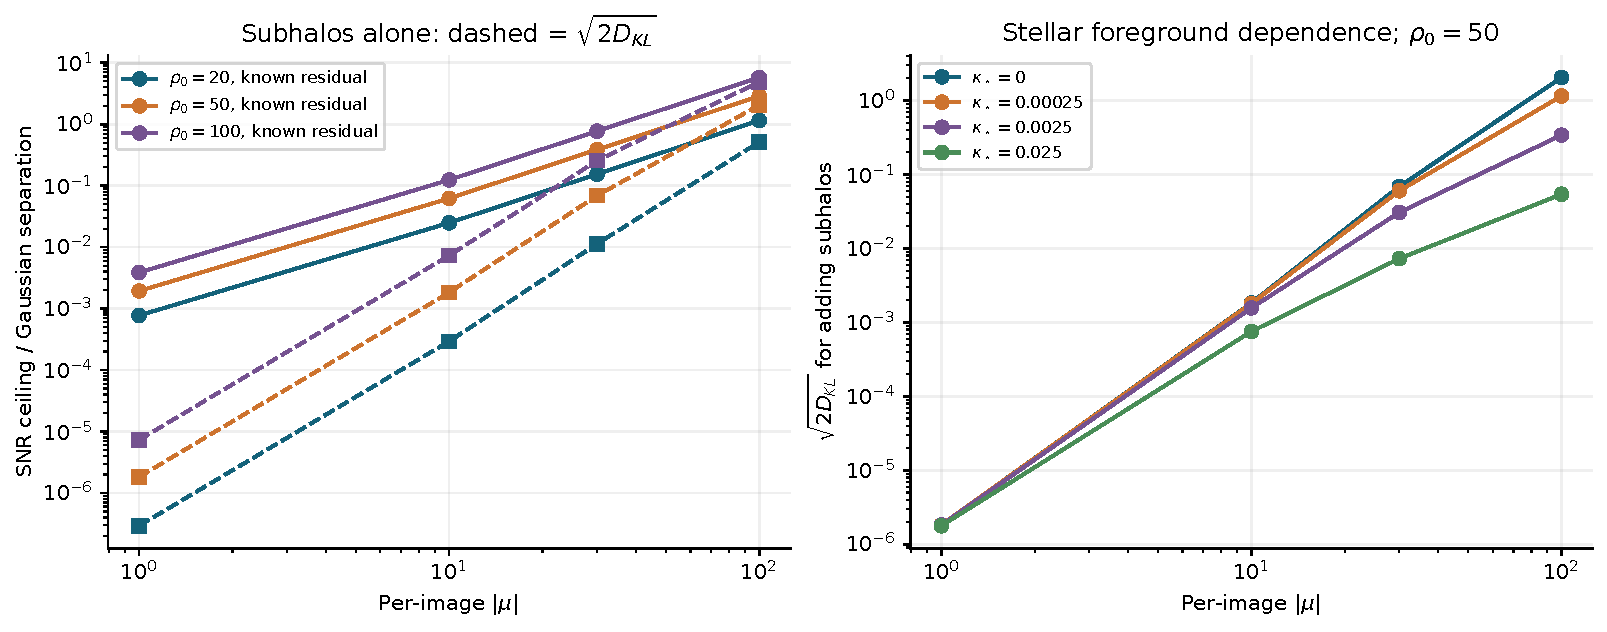
\includegraphics[width=\linewidth]{covariance_detectability.pdf}
\caption{Left: known-realization residual SNR (solid) and subhalo-only Gaussian
covariance separation (dashed) for several unlensed in-band SNRs. Right: the
dependence on stellar surface convergence at $\rho_0=50$, after marginalizing
stellar realizations while fixing their covariance. The ordinate is information
separation, not a $p$-value or a detection significance.}
\end{figure}

\begin{figure}[htbp]
\centering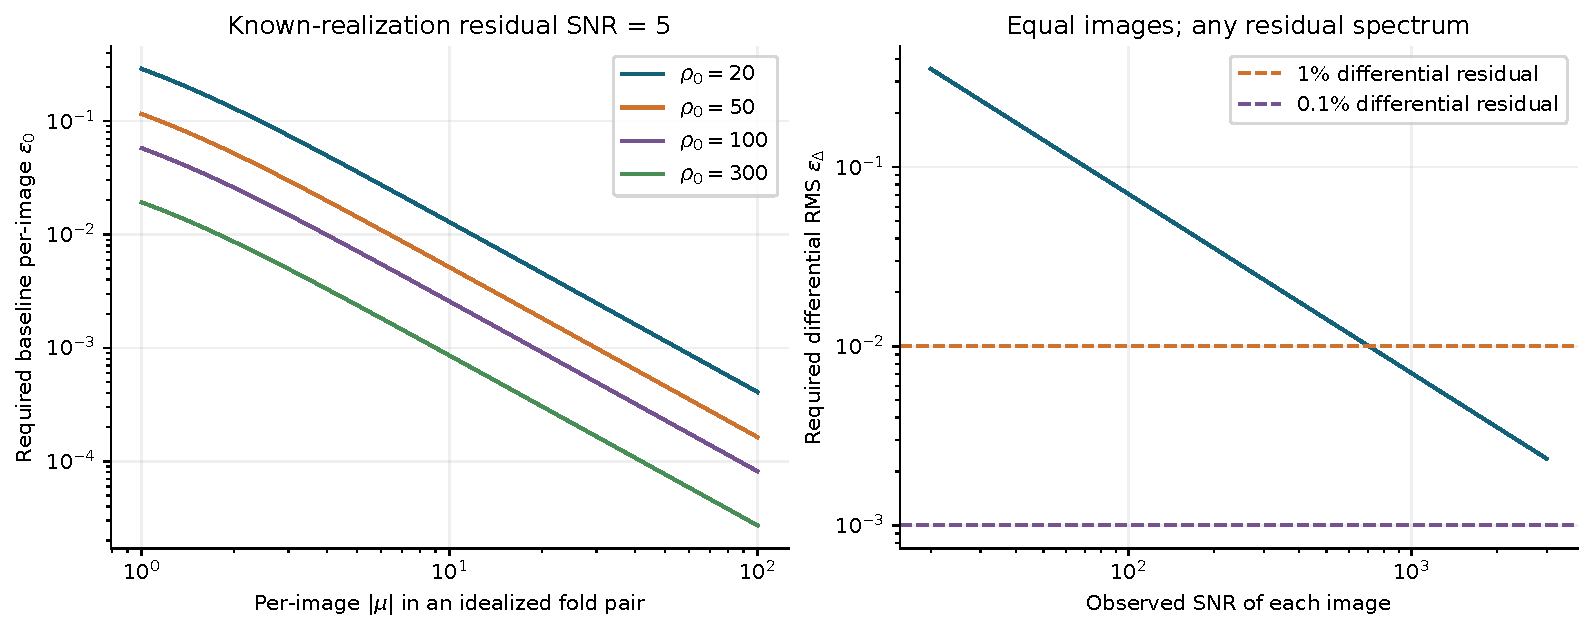
\includegraphics[width=\linewidth]{snr_requirements.pdf}
\caption{Sensitivity requirements independent of a particular detector.
Left: the conditional $n=-2$ scale-free model, where $\epsilon_0$ is the
baseline per-image projected RMS and the two images are independent.
Right: the required \emph{differential} RMS for equally loud images with any
specified residual shape. A known-realization SNR of five is a sensitivity
reference, not a claim of five-sigma stochastic detection.}
\end{figure}

For the scale-free $n=-2$ example, the independent fold-pair ceiling can be
written particularly simply:
\begin{equation}
 \rho_{\rm res,rms}=\rho_0\epsilon_0
 \sqrt{\frac{3}{8}|\mu|\left(|\mu|^2+1\right)}.
\end{equation}
This is useful for exploring future sensitivities without inventing a
fourth-generation design curve. Large magnifications are rare: the local fold
mapping gives an unbiased source-plane cross-section above $|\mu|$ proportional
to $|\mu|^{-2}$. Magnification bias, the population, time delays, detectability
of both images, and microcaustics must be included before quoting event rates.

\begin{figure}[htbp]
\centering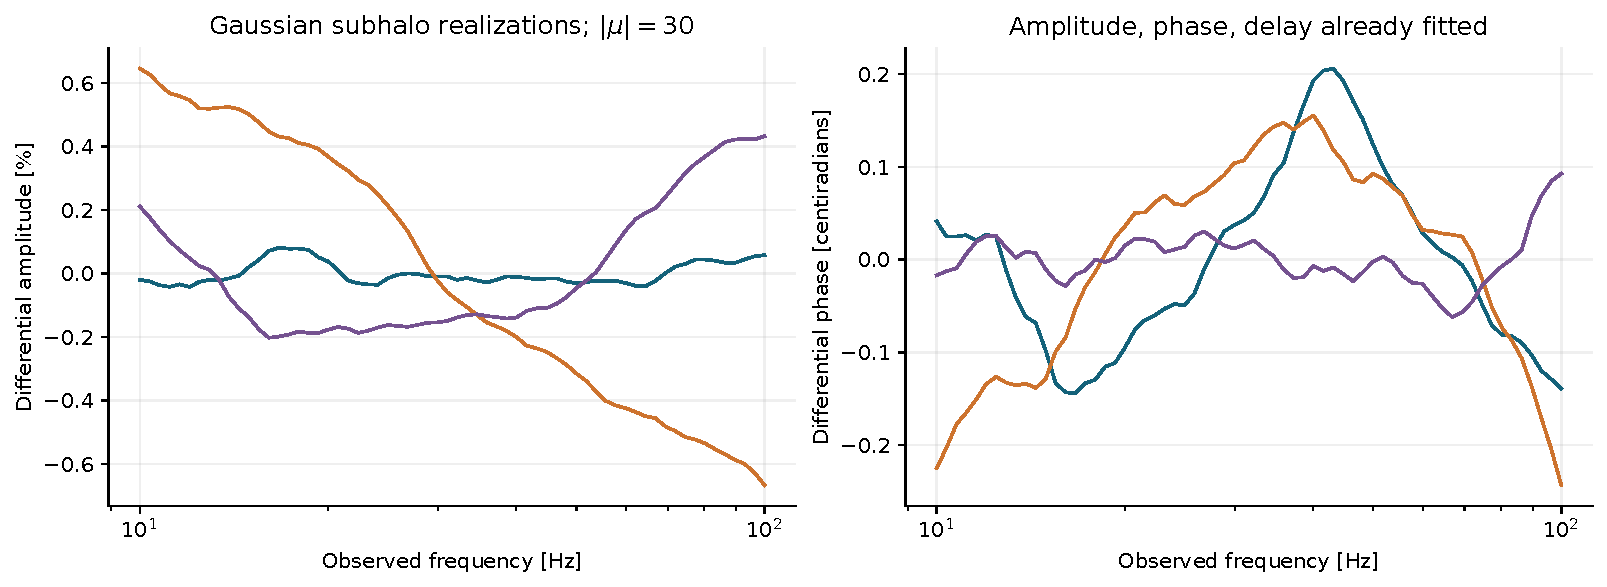
\includegraphics[width=\linewidth]{example_residuals.pdf}
\caption{Three seeded Gaussian realizations from the calculated real joint
subhalo covariance at $|\mu|=30$. These are illustrative random weak-screen
signals, not waveform simulations or individual halo ray-tracing results.
The fitted magnification, phase, and arrival time have already been removed.}
\end{figure}
\FloatBarrier

\section{Audit of the earlier LISA-to-ground-band extrapolation}
\label{sec:figure-audit}

The raw variance in Eq.~(7) of Ref.~\cite{choi2026} includes the geometric
contribution $H\to1$ from low wavenumber. For $P_\kappa\propto k^{-2}$ it
has an infrared logarithm. It is therefore not generally localized to the
Fresnel scale, and its value cannot be inferred from a single plotted power
value. A projected residual is the appropriate quantity.

We separately extract the vector path of the lowest-mass-cut curve in Fig.~2
of the version-1 PDF. The independent digitization script records a source
hash, axis fits, curve selection, and validation. It yields approximate plotted
values $P_\kappa\simeq5.4\times10^{-14}$ at equivalent frequency $0.01$ Hz
and $2.0\times10^{-19}$ at $100$ Hz. These are the figure's dimensionless
normalization, not measured waveform variances. Their high-wavenumber slope is
$n\simeq-2.71$, rather than $-2$.

For an ideal power law spanning the relevant kernels and identically scaled
frequency weights, Eq.~\eqref{eq:powerlaw-scaling} gives
\begin{equation}
 \frac{\sigma_\perp(100\,\mathrm{Hz})}{\sigma_\perp(0.01\,\mathrm{Hz})}
 \sim(10^4)^{(-2.71+2)/4}\simeq0.2.
\end{equation}
This is a slope-based estimate, not a full LIGO/LISA comparison. The figure's
top axis maps physical scale to frequency for a reference lens at $z_l=1$;
its spectrum already integrates along the line of sight to $z_s=2$.
The curve is simplified in the PDF and is not the authors' numerical data.
We do not use its absolute normalization in the independent local-lens model.
The earlier conclusion of comparable amplitudes should therefore be withdrawn.

\section{Validation, scope, and the next physical calculation}

The unit tests check the unlensed and geometric kernel limits, the exact
power-law macro gain, real nuisance projection, covariance positivity and
null directions, NFW transforms against radial quadrature, mass normalization,
harmonic image weights, and both weak- and finite-signal likelihood limits.
The independent convergence script doubles radial, angular, and frequency
sampling for selected cases, compares covariance traces against direct
variance integration, and checks the infrared cutoff needed for the mHz scan.
The numerical reports are committed with the figures and code.

The work is complete as a reproducible exploratory calculation. A physical
forecast still requires the following distinct inputs:
\begin{enumerate}
\item A specified detector/network response and redshifted BBH population,
including selection on the SNR of \emph{both} images and observing time.
\item A calibrated, tidally evolved subhalo population in galaxy and cluster
lenses, with survival and concentration uncertainties at the relevant scales.
\item Stellar and remnant mass distributions with nonlinear diffraction tests
in the configurations where the weak-screen model becomes marginal.
\item Multiplane propagation and inter-image correlations for field halos
away from the primary lens plane; they cannot be multiplied by the same
local macro gain without derivation.
\item A network likelihood for shared source polarizations, calibration,
macro nuisance parameters, and non-Gaussian small-scale lens realizations.
\end{enumerate}

These requirements specify what would turn an enhanced diffraction signal into
a credible dark-matter inference. They also suggest a focused follow-up:
compare low-stellar-density cluster image pairs with ordinary galaxy pairs,
using the same in-band SNR and a realistic subhalo-survival model.

\bibliographystyle{unsrt}
\bibliography{references,systematics_references,consistency_references}
\end{document}
